\documentclass[10pt, twoside]{article}
\usepackage{fancyhdr}
\usepackage{amsmath, amsthm, amssymb}
\usepackage[catalan]{babel}
\usepackage[titles]{tocloft}
\usepackage[utf8]{inputenc}
\usepackage[left=2.15cm, right=2.15cm, top=30mm, bottom=20mm]{geometry}
\usepackage{parskip}
\setlength{\parindent}{0pt} % Elimina la sangría de la primera línea de cada párrafo
\usepackage{titlesec}
\usepackage{bookmark}
\usepackage{multirow}
\usepackage{graphicx}
\usepackage{physics}
\usepackage{hyperref}
\usepackage{float}
\usepackage{caption}
\usepackage{booktabs}

\captionsetup{labelfont=bf}


\begin{document}

\begin{titlepage}
\centering
{\Large Fonaments d'Enginyeria Química \\ MO70399 \par}
\vspace{2cm}
{\Huge \textbf{Pràctica 2:} \par}
\vspace{1cm}
{\Huge \textbf{Balanç d'energia calorífica} \par}
\vspace{2cm}
{\Large Grup B \par}
\vspace{0.5cm}
{\Large Torn 2 \par}
\vspace{0.5cm}
{\normalsize Baldi Garcia, Isaac: 1667260 \\ Barbens Calzadilla, Carla: 1666167 \\ Belmonte Leiva, Marc: 1619451 \\ Bujones Umbert, Jun Shan: 1549086 \\ Franco Avilés, Eric: 1666739 \\ Gómez Rubio, Miquel: 1668850 \\ González Barea, Eric: 1672980 \\ Jacas García, Eira: 1666616\par}
\vspace{2cm}
{\normalsize 6 pàgines \par}
{\Large Gener 2025 \par}
\vspace{1cm}

\includegraphics[width=0.4\textwidth]{Logo_UAB.png}


\end{titlepage}

\pagenumbering{gobble}
\renewcommand{\cftsecfont}{}
\renewcommand{\cftsecpagefont}{}
\renewcommand{\cftsecleader}{\cftdotfill{\cftdotsep}}
\renewcommand{\cftdotsep}{0.2}
\setlength{\cftbeforesecskip}{0.5em}
\setlength{\cftbeforesubsecskip}{0.5em}
\tableofcontents

\newpage
\pagenumbering{arabic}
\setcounter{page}{1}

\pagestyle{fancy}
\lhead{\textbf{Pràctica 2: Balanç d'energia calorífica}}
\rhead{\textbf{Fonaments d'Enginyeria Química}}

\begin{abstract}
En aquesta pràctica ens proposem estudiar els balanços d'energia calorífica aplicats a un tanc adiabàtic, en el qual no es produeix cap tipus d'intercanvi d'energia i/o matèria, i en concret de calor, amb l'entorn.  Per tal de demostrar experimentalment això, mesurarem la temperatura de l'aigua que flueix per dins del reactor en diferents temps, comparant-los amb la temperatura del tanc pulmó.
\end{abstract}

\section{Calibratge de la bomba i mesura del volum del tanc}
Abans de començar amb la part experimental cal que, prèviament, calibrem la bomba, per tal de conèixer quins cabals es corresponen amb cada valor de rpm's de la bomba, i mesurem el volum del tanc. S'han obtingut els següents valors.
\subsection{Calibratge de la bomba}

\begin{table}[h!]
    \centering
    \caption{Resultats obtinguts en el calibratge de la bomba.}
    \label{tab1}
    \begin{tabular}{|c|c|c|} % Estructura de columnas
    \hline
    Revolucions per minut (rpm) & Volum (mL) & Cabal (mL/min) \\ \hline
    90       & 625       & 205,33       \\ \hline
    110      & 760       & 253,33       \\ \hline
    130      & 910       & 303,33       \\ \hline
    \end{tabular}
\end{table}
 
\begin{figure}[h]
    \centering
    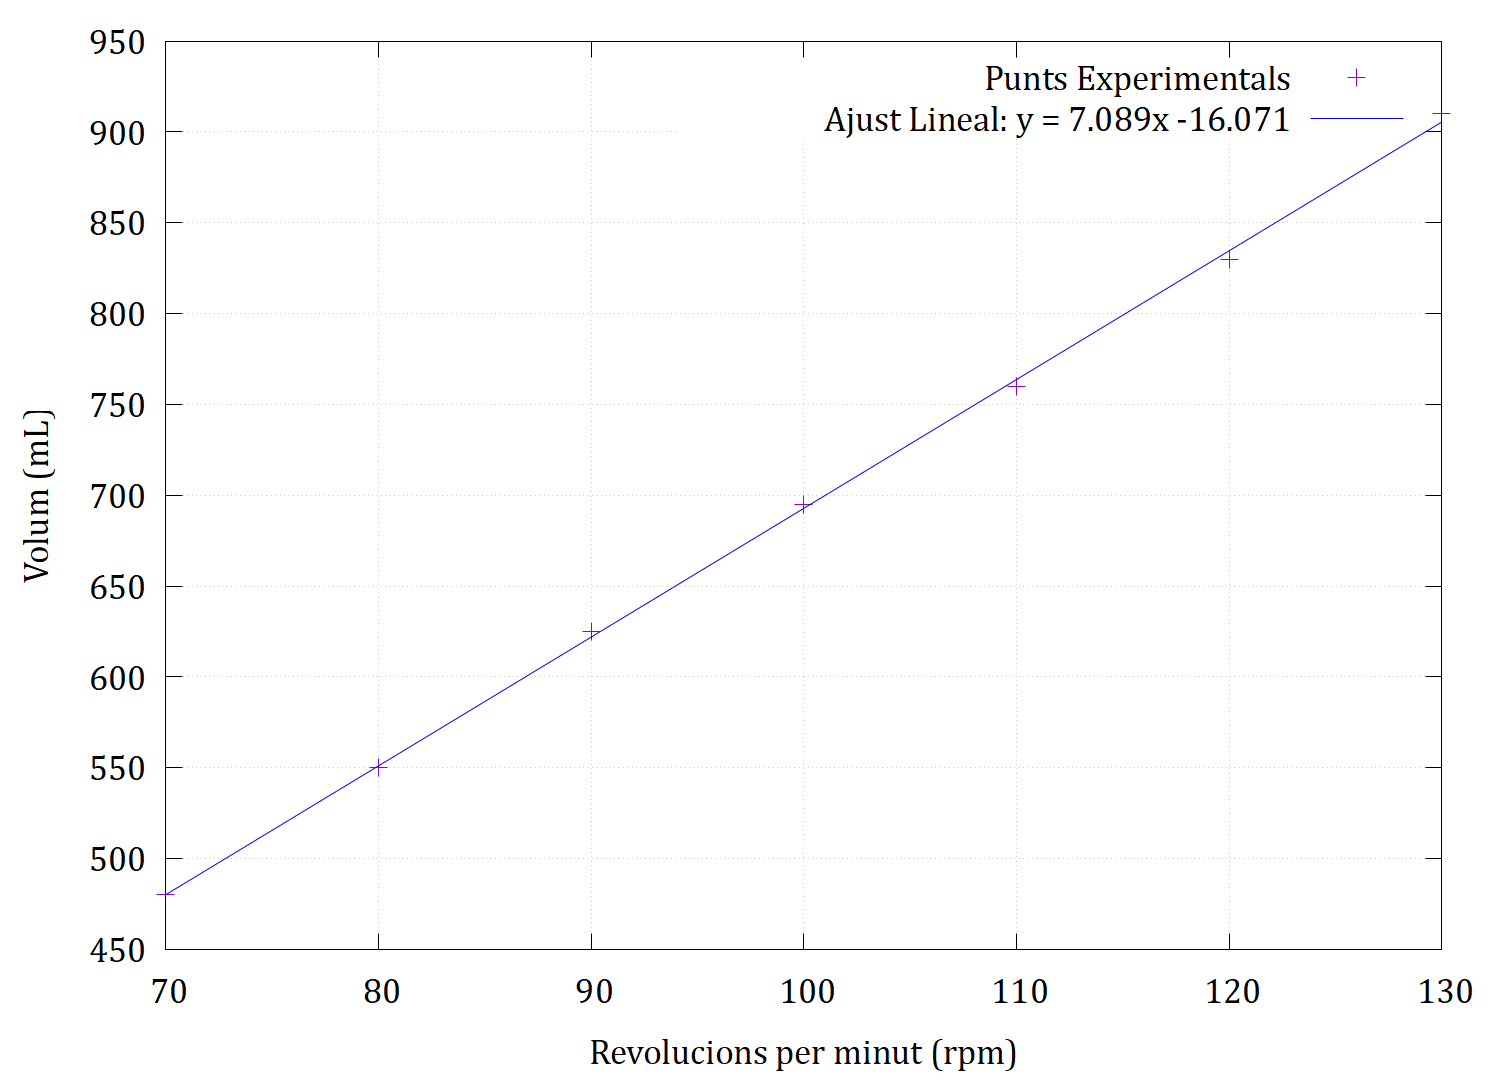
\includegraphics[width=0.7\linewidth]{calbombagnu.png}
    \caption{Corba de calibratge per la bomba}
    \label{fig1}
\end{figure}
 
\subsection{Mesura del volum del tanc}
Els volums trobats trobats usant els dos mètodes proposats és\footnote{A l'annex s'explica en què consisteix cadascun dels dos mètodes.}:
\begin{itemize}
    \item \textbf{Mètode 1: }El volum obtingut ha estat $\Rightarrow$ $\boxed{V = 1595,00 \text{ mL}}$.
    \item \textbf{Mètode 2: }El volum obtingut ha estat $\Rightarrow$ $\boxed{V = 1637,98 \text{ mL}}$.
    \item \textbf{Volum promig: }El volum promig obtingut ha estat $\Rightarrow$ $\boxed{V = 1616,49 \text{ mL}}$.
\end{itemize}

\subsection{Mesures de temperatura}
A continuació adjuntem les mesures de temperatura pels 3 cabals proposats. A l'annex C comentem la metodologia seguida per tal de fer la presa de dades.

Les temperatures inicials del tanc i del pulmó per a cada cas han estat:

\begin{table}[h!]
    \centering
    \caption{Temperatures inicials del tanc i del pulmó per cada valor $Q_L$.}
    \begin{tabular}{cccc}
        \toprule
        & $Q_L = 203.33$ mL/min & $Q_L = 253,33$ mL/min & $Q_L = 303,33$ mL/min \\
        \midrule
        \textbf{T$_0$ al Tanc (K)} & 362,0 & 364,1 & 364,6 \\
        \textbf{T del Pulmó (K)}  & 290,6 & 290,3 & 290,1 \\
        \bottomrule
    \end{tabular}
    \label{tabla:temperaturas}
\end{table}

Tot seguit adjuntem 3 taules (una per cada cabal) amb totes les temperatures mesurades:
\begin{table}[H]
    \centering
    \begin{minipage}{0.3\textwidth}
        \centering
        \caption{Resultats experimentals amb $Q_L = 203,33 \frac{\text{mL}}{\text{min}}$.}
        \begin{tabular}{ccc}
            \toprule
            \textbf{Temps (s)} & \textbf{T (ºC)} & \textbf{T (K)} \\
            \midrule
            0   & 88,8 & 362,0 \\
            30  & 88,4 & 361,6 \\
            60  & 87,2 & 360,4 \\
            90  & 85,7 & 358,9 \\
            120 & 82,7 & 355,9 \\
            150 & 78,3 & 351,5 \\
            180 & 73,2 & 346,4 \\
            210 & 69,0 & 342,1 \\
            240 & 65,3 & 338,5 \\
            270 & 61,2 & 334,4 \\
            300 & 57,9 & 331,1 \\
            330 & 54,5 & 327,7 \\
            360 & 51,2 & 324,4 \\
            390 & 48,3 & 321,5 \\
            420 & 46,1 & 319,3 \\
            450 & 43,7 & 316,9 \\
            480 & 41,5 & 314,7 \\
            510 & 39,4 & 312,6 \\
            540 & 36,7 & 309,9 \\
            570 & 35,6 & 308,8 \\
            600 & 34,0 & 307,2 \\
            
            \bottomrule
        \end{tabular}
        
        \label{tabla:muestra1}
    \end{minipage}%
    \hfill
    \begin{minipage}{0.3\textwidth}
        \centering
        \caption{Resultats experimentals amb $Q_L = 253,33 \frac{\text{mL}}{\text{min}}$.}
        \begin{tabular}{ccc}
            \toprule
            \textbf{Temps (s)} & \textbf{T (ºC)} & \textbf{T (K)} \\
            \midrule
            0   & 90,9 & 364,1 \\
            30  & 90,3 & 363,5 \\
            60  & 88,2 & 361,4 \\
            90  & 83,4 & 356,6 \\
            120 & 77,5 & 350,7 \\
            150 & 72,2 & 345,4 \\
            180 & 66,7 & 339,9 \\
            210 & 61,5 & 334,7 \\
            240 & 56,8 & 330,0 \\
            270 & 53,7 & 326,9 \\
            300 & 51,0 & 324,2 \\
            330 & 48,0 & 321,2 \\
            360 & 44,9 & 318,1 \\
            390 & 42,4 & 315,6 \\
            420 & 39,8 & 313,0 \\
            450 & 39,4 & 312,6 \\
            480 & 37,1 & 310,3 \\
            510 & 35,6 & 308,8 \\
            540 & 34,4 & 307,6 \\
            570 & 33,2 & 306,4 \\
            - & - & - \\
            \bottomrule
        \end{tabular}
        \label{tabla:muestra2}
    \end{minipage}%
    \hfill
    \begin{minipage}{0.3\textwidth}
        \centering
        \caption{Resultats experimentals amb $Q_L = 303,33 \frac{\text{mL}}{\text{min}}$.}
        \begin{tabular}{ccc}
            \toprule
            \textbf{Temps (s)} & \textbf{T (ºC)} & \textbf{T (K)} \\
            \midrule
            0   & 91,4 & 364,6 \\
            30  & 86,2 & 359,4 \\
            60  & 82,8 & 356,0 \\
            90  & 77,5 & 350,7 \\
            120 & 71,0 & 344,2 \\
            150 & 64,5 & 337,7 \\
            180 & 61,1 & 334,3 \\
            210 & 56,4 & 329,6 \\
            240 & 53,7 & 326,9 \\
            270 & 50,4 & 323,6 \\
            300 & 47,4 & 320,6 \\
            330 & 45,0 & 318,2 \\
            360 & 42,5 & 315,7 \\
            390 & 40,5 & 313,7 \\
            420 & 38,6 & 311,8 \\
            450 & 36,7 & 309,9 \\
            480 & 35,0 & 308,2 \\
            510 & 33,4 & 306,6 \\
            - & - & - \\
            - & - & - \\
            - & - & - \\
            \bottomrule
        \end{tabular}
        
        \label{tabla:muestra3}
    \end{minipage}
\end{table}

\section{Resultats experimentals i discussió}

\subsection{Temperatures teòriques vs. experimentals}
En aquest apartat compararem, per a cada cabal treballat, les temperatures experimentals respecte les teòriques, aquestes últimes calculades segons l'equació (que podeu trobar al guió de la pràctica):
\begin{equation}
    T(t)=T_1+(T_0-T_1)\text{ exp}\left(-\frac{Q_L}{V}t\right)
\end{equation}

\begin{figure}[h!]
    \centering
    \begin{minipage}{0.45\linewidth}
        \centering
        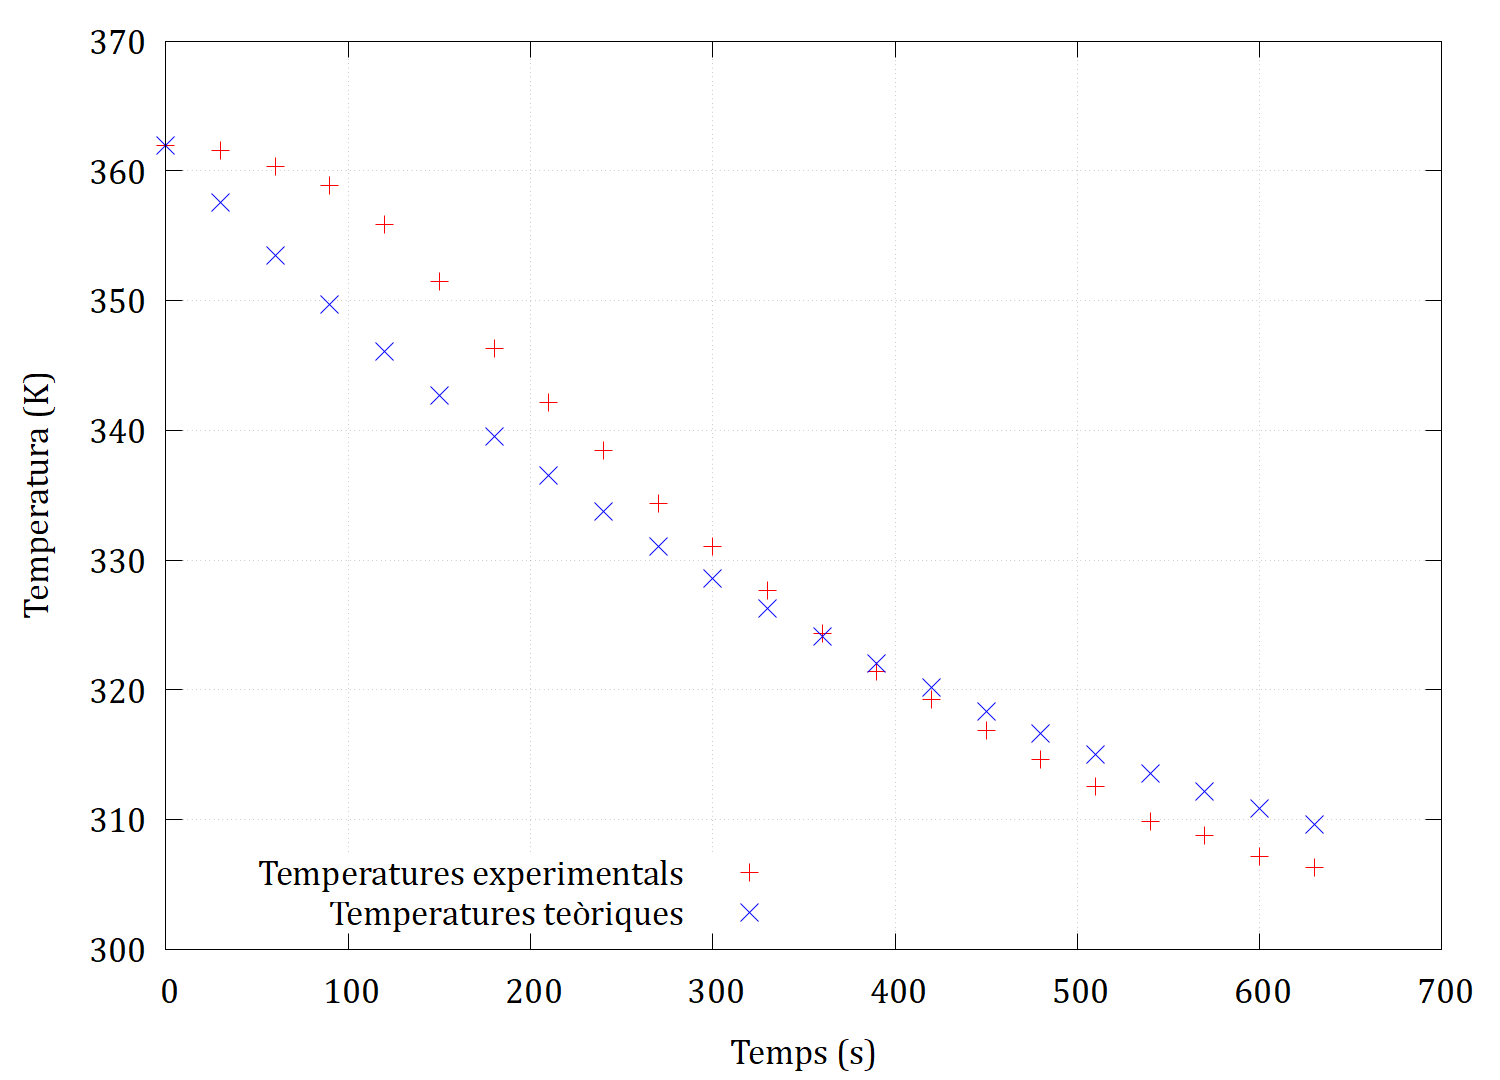
\includegraphics[width=\linewidth]{203.png}
        \caption{Evolució de les temperatures teòriques i experimentals pel cabal de 203,33 mL/min.}
    \end{minipage}
    \hspace{0.05\linewidth}
    \begin{minipage}{0.45\linewidth}
        \centering
        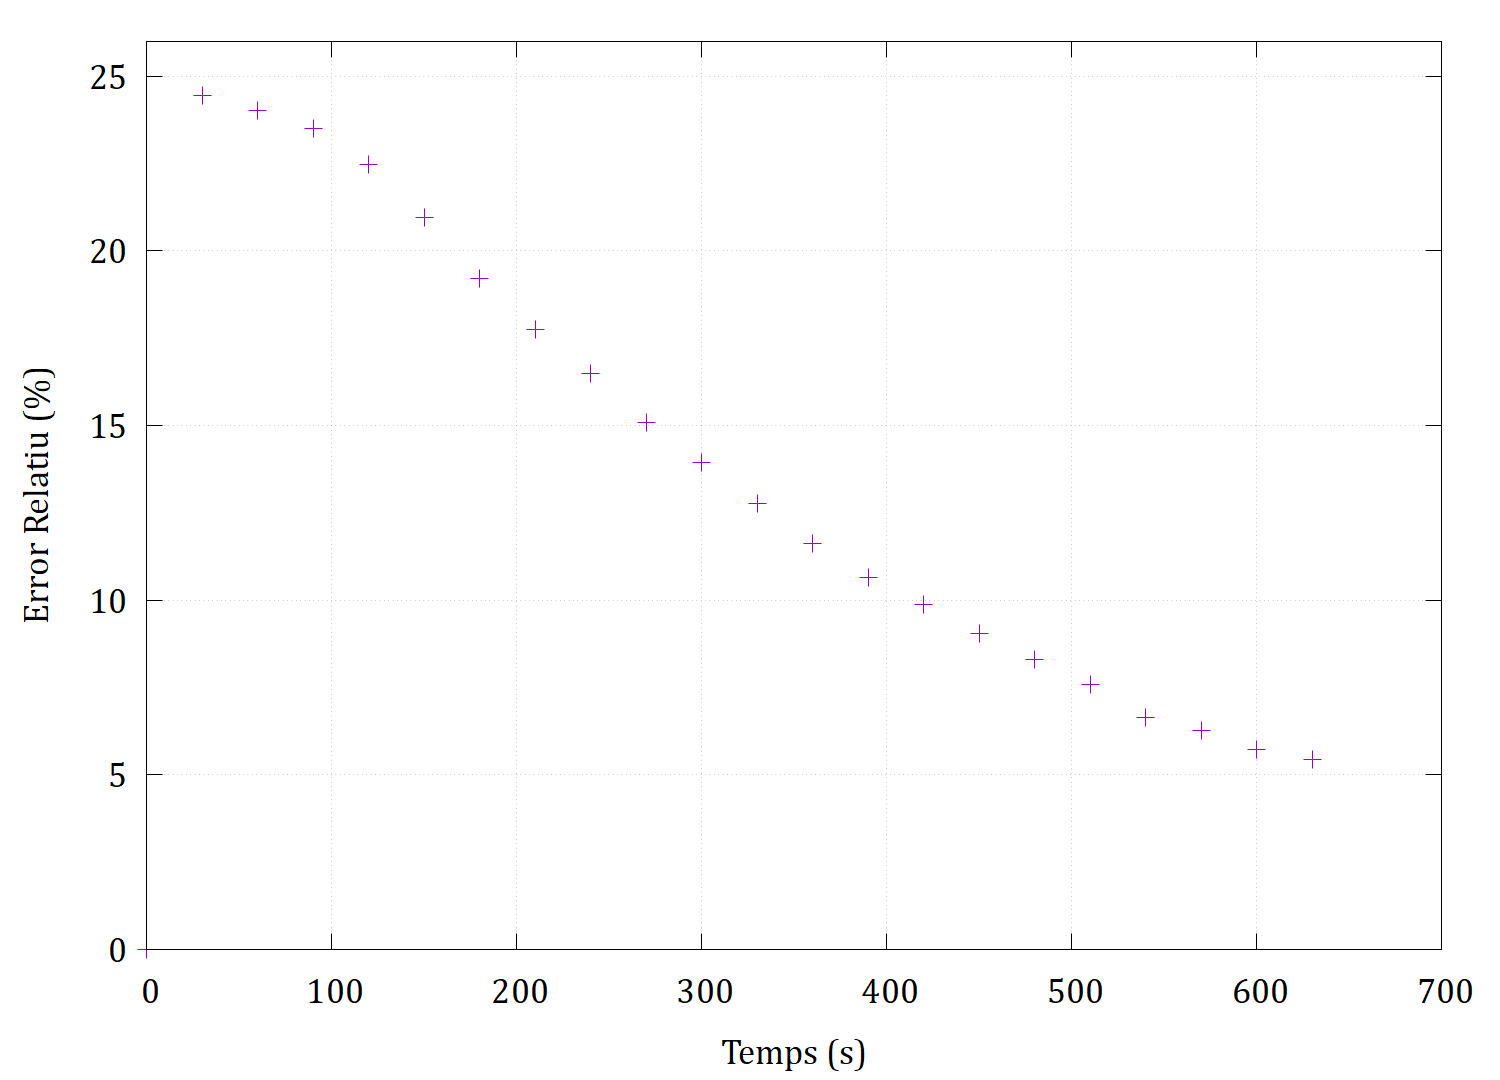
\includegraphics[width=\linewidth]{203error.png}
        \caption{Error relatiu de la temperatura experimental respecte la teòrica pel cabal de 203,33 mL/min.}
    \end{minipage}
\end{figure}

\begin{figure}[h!]
    \centering
    \begin{minipage}{0.45\linewidth}
        \centering
        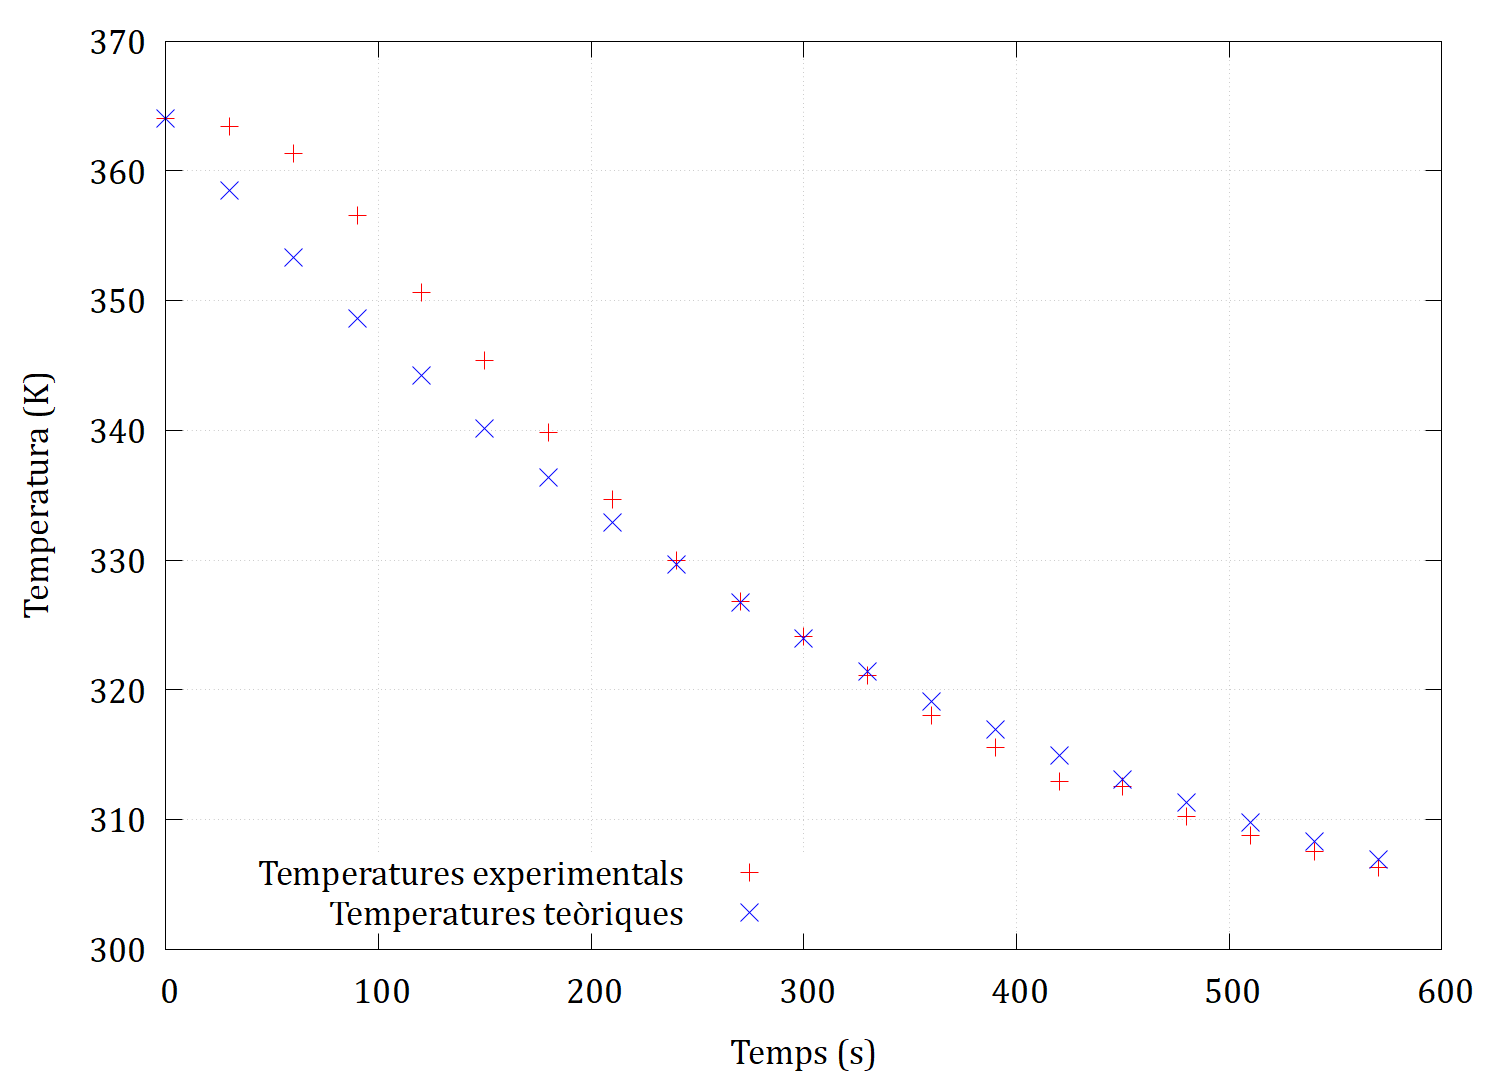
\includegraphics[width=\linewidth]{253.png}
        \caption{Evolució de les temperatures teòriques i experimentals pel cabal de 253,33 mL/min.}
    \end{minipage}
    \hspace{0.05\linewidth}
    \begin{minipage}{0.45\linewidth}
        \centering
        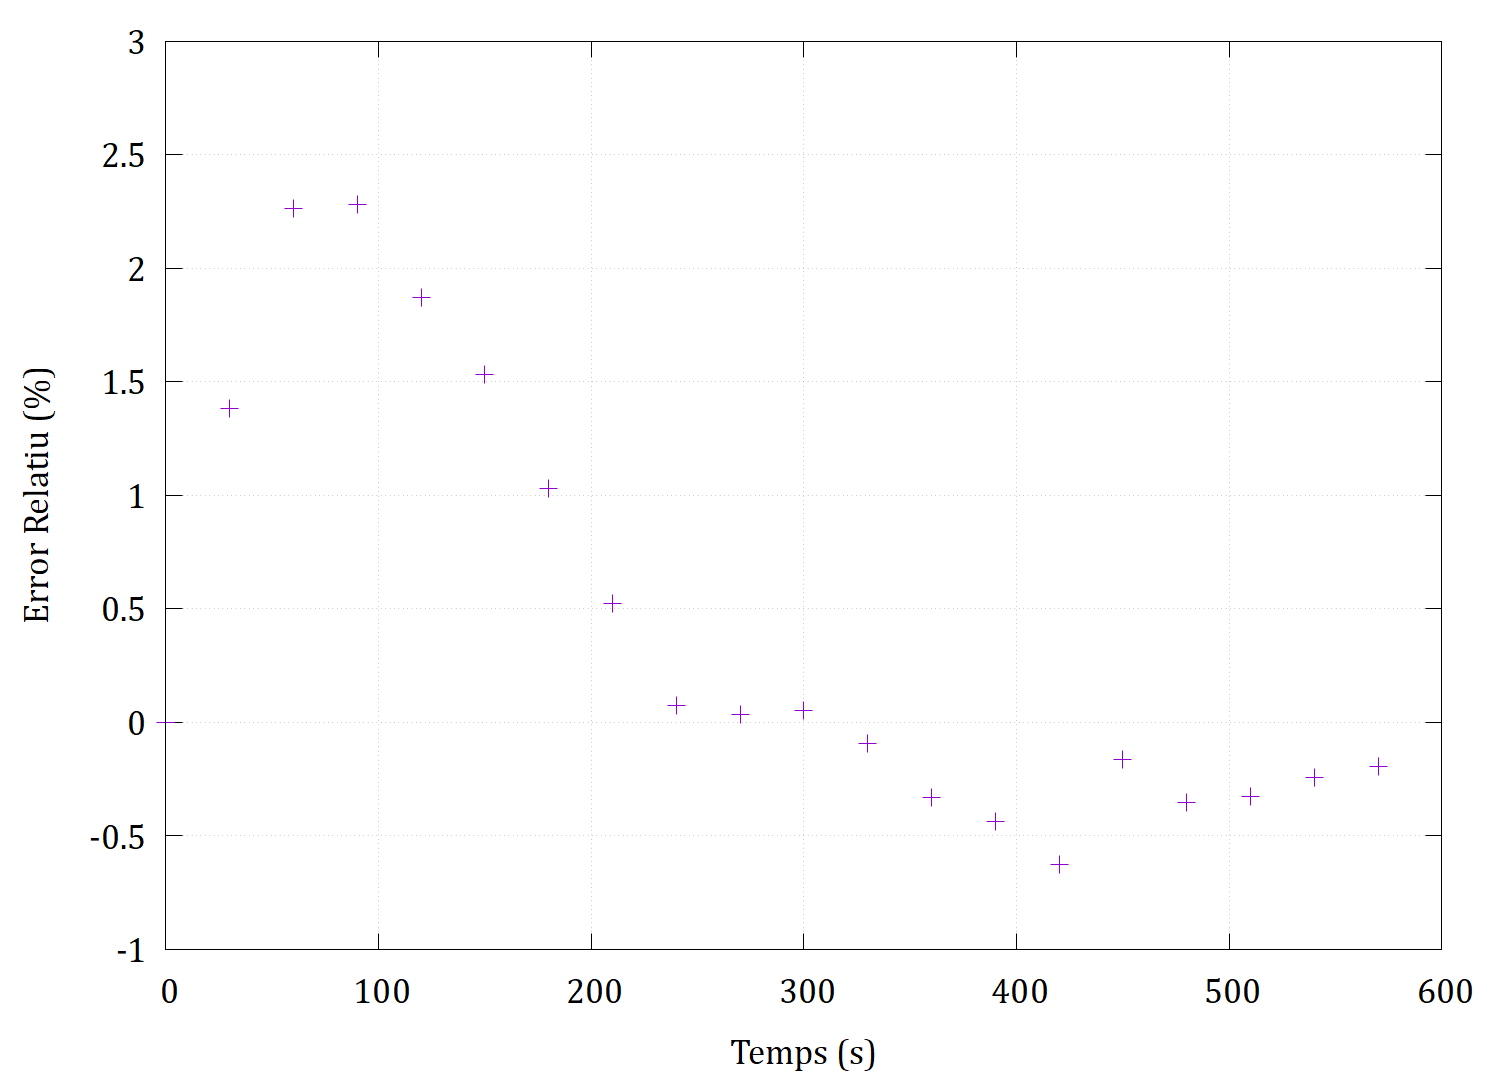
\includegraphics[width=\linewidth]{253error.png}
        \caption{Error relatiu de la temperatura experimental respecte la teòrica pel cabal de 253,33 mL/min.}
    \end{minipage}
\end{figure}

\begin{figure}[H]
    \centering
    \begin{minipage}{0.45\linewidth}
        \centering
        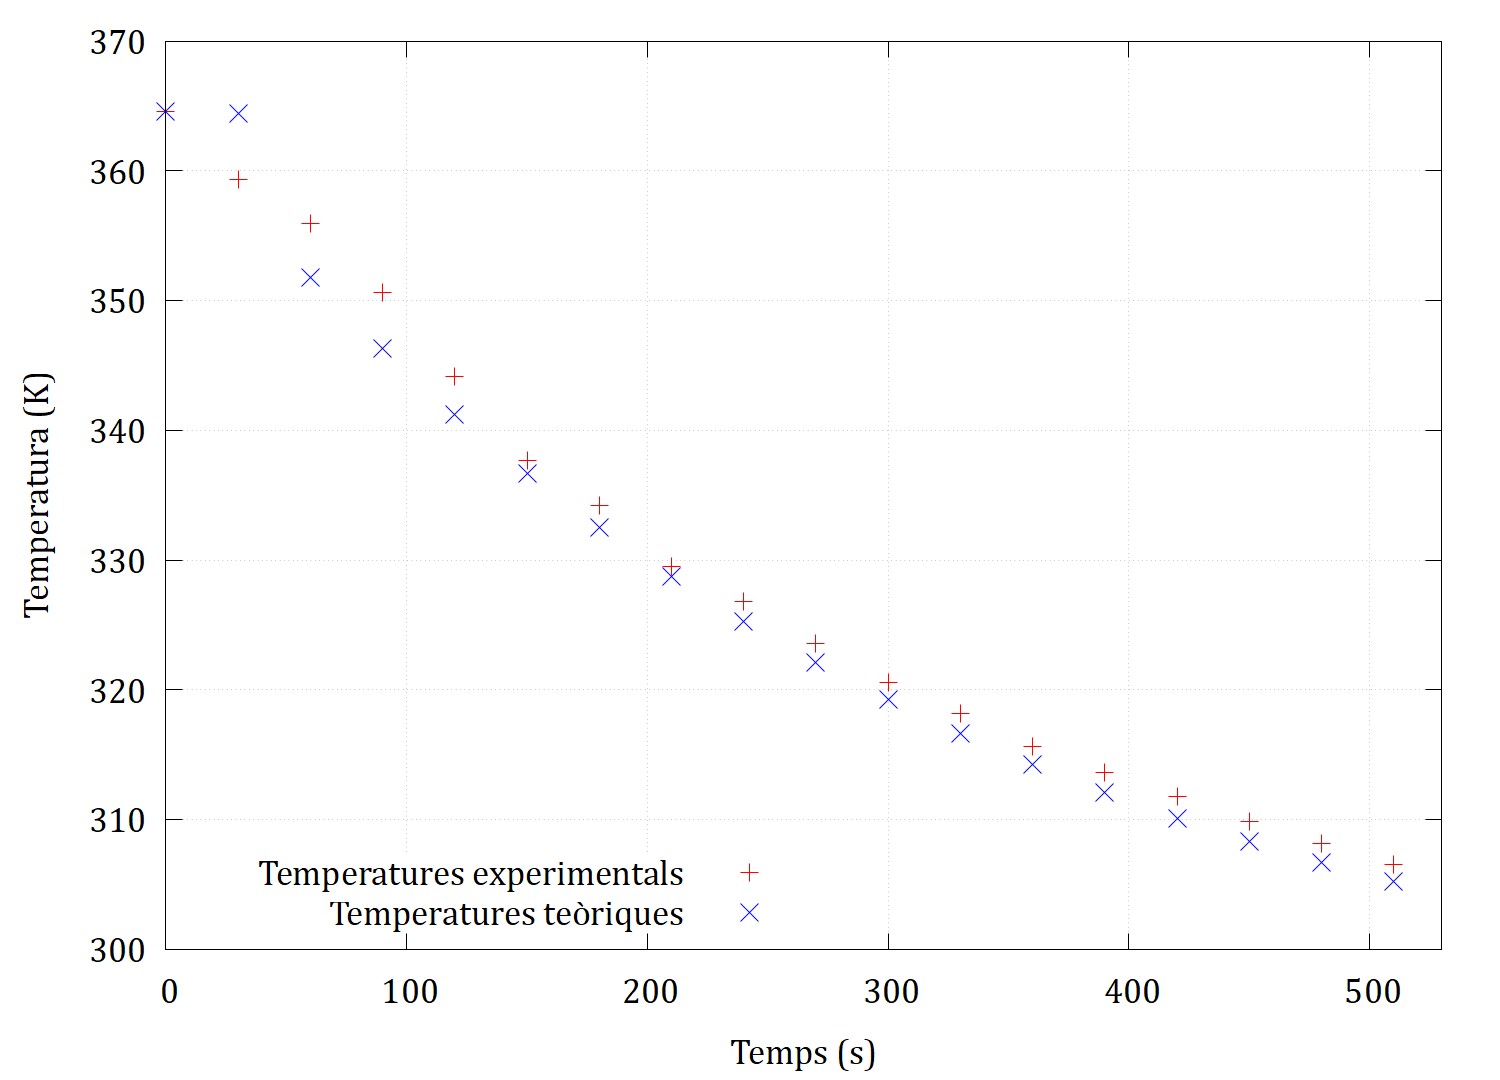
\includegraphics[width=\linewidth]{303.png}
        \caption{Evolució de les temperatures teòriques i experimentals pel cabal de 303,33 mL/min.}
    \end{minipage}
    \hspace{0.05\linewidth}
    \begin{minipage}{0.45\linewidth}
        \centering
        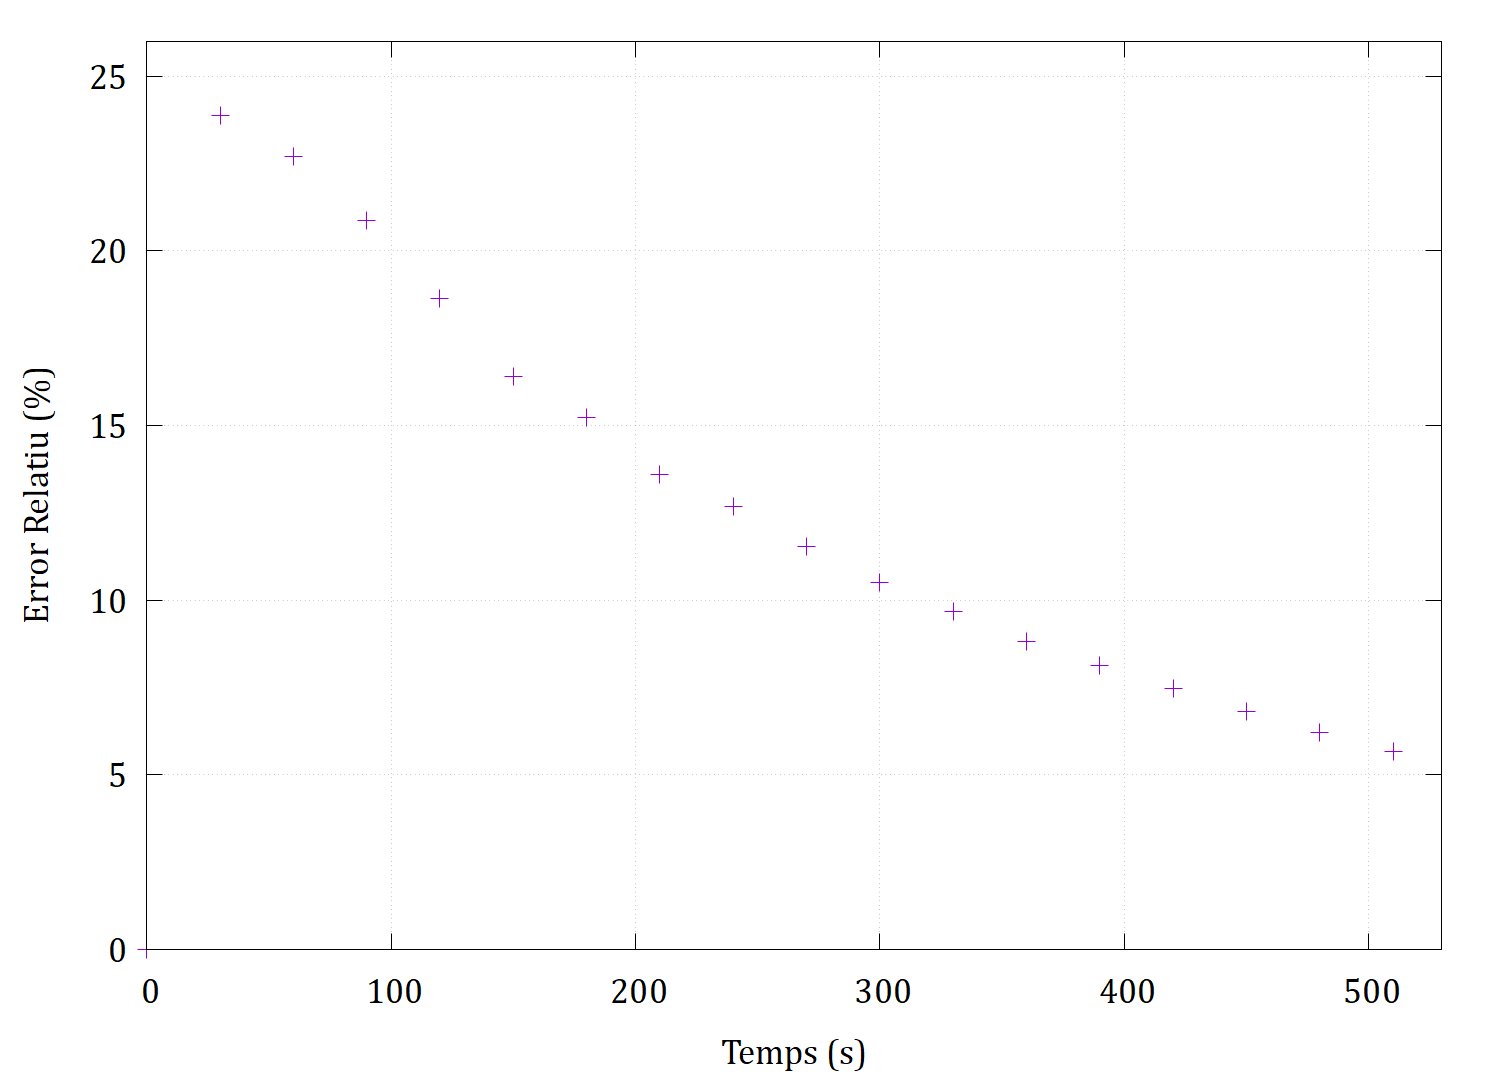
\includegraphics[width=\linewidth]{303error.png}
        \caption{Error relatiu de la temperatura experimental respecte la teòrica pel cabal de 303,33 mL/min.}
    \end{minipage}
\end{figure}

Observant les figures 2, 4 i 6 notem ràpidament que hem obtingut valors de temperatura experimentals semblants als esperats. Per corroborar-ho, podem fixar-nos en les figues 3, 5 i 7 que mostren l'error relatiu (en percentatge) comès a cada mesura, sent el màxim un 3\%.

\subsection{Representació semilogarítmica de les temperatures experimentals}
PartiM de l'equació linealitzada: 
\begin{equation}
    \log(T') = \log(T'_0) - \frac{Q_L}{2,303V} t
\end{equation}
Representem gràficament el logaritme de les temperatures experimentals menys la temperatura del tanc pulmó respecte el temps per cadascun dels cabals utilitzats durant l'experiment.

\begin{figure}[h!]
    \centering
    \begin{minipage}{0.45\linewidth}
        \centering
        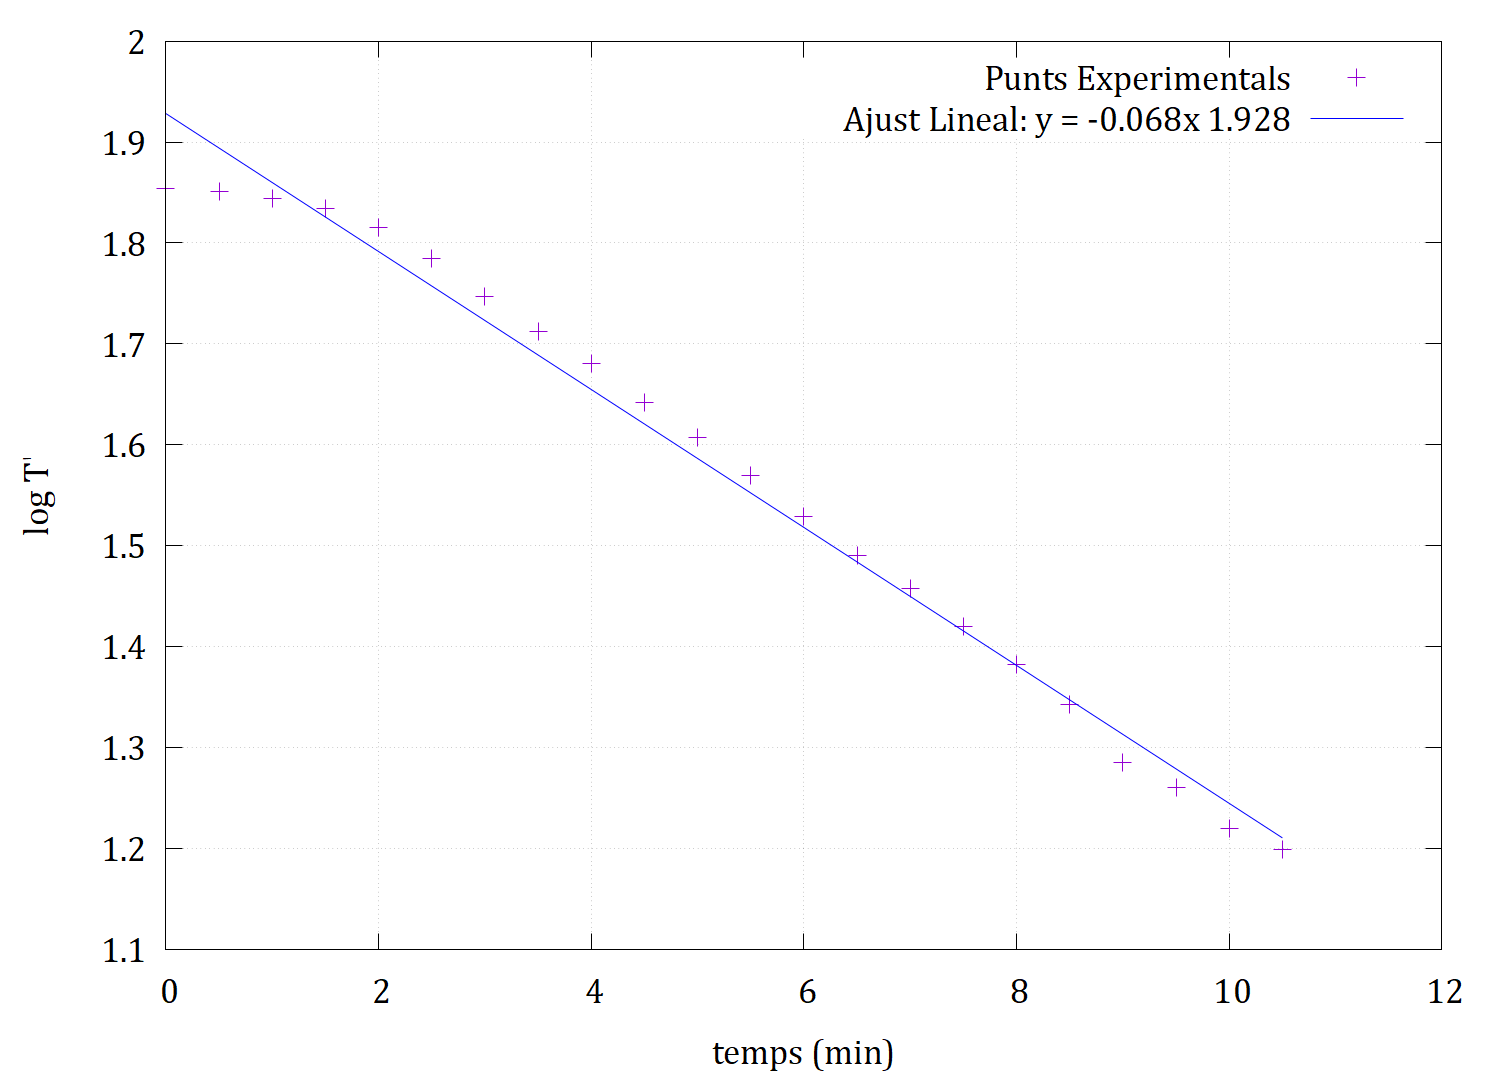
\includegraphics[width=\linewidth]{ajustsemilog203.png}
        \caption{Gràfic semilogarítmic pel cabal 203,33 mL/min.}
    \end{minipage}
    \hspace{0.05\linewidth}
    \begin{minipage}{0.45\linewidth}
        \centering
        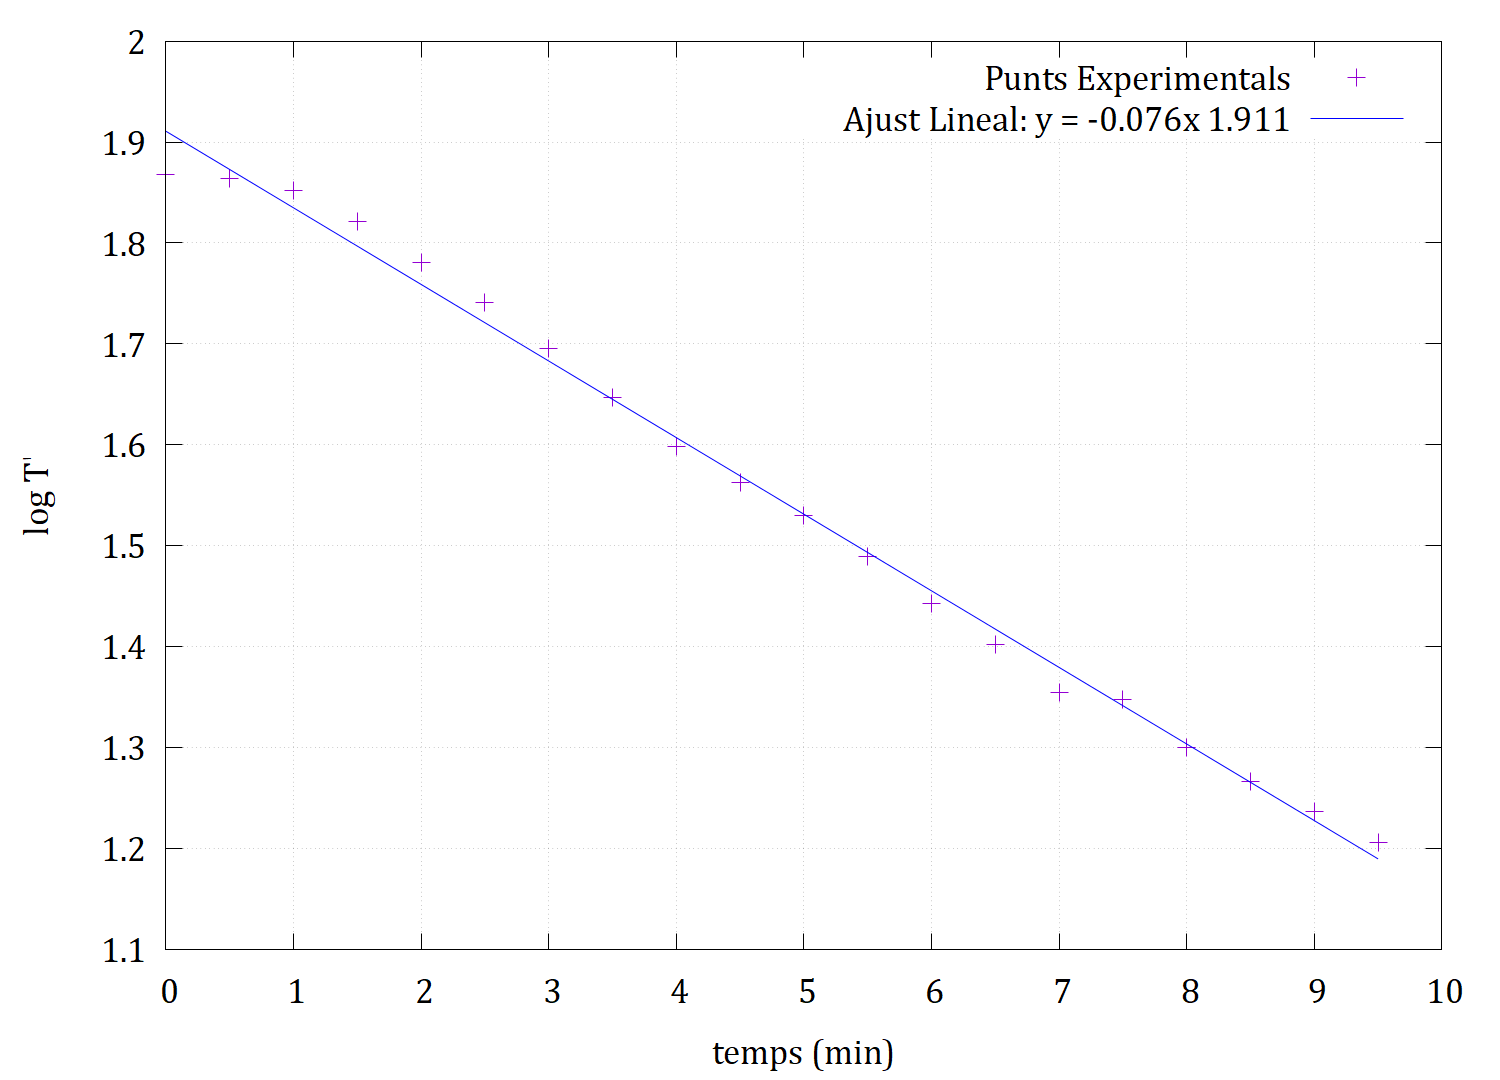
\includegraphics[width=\linewidth]{ajustsemilog253.png}
        \caption{Gràfic semilogarítmic pel cabal 203,33 mL/min.}
    \end{minipage}
\end{figure}

\begin{figure}[H]
    \centering
    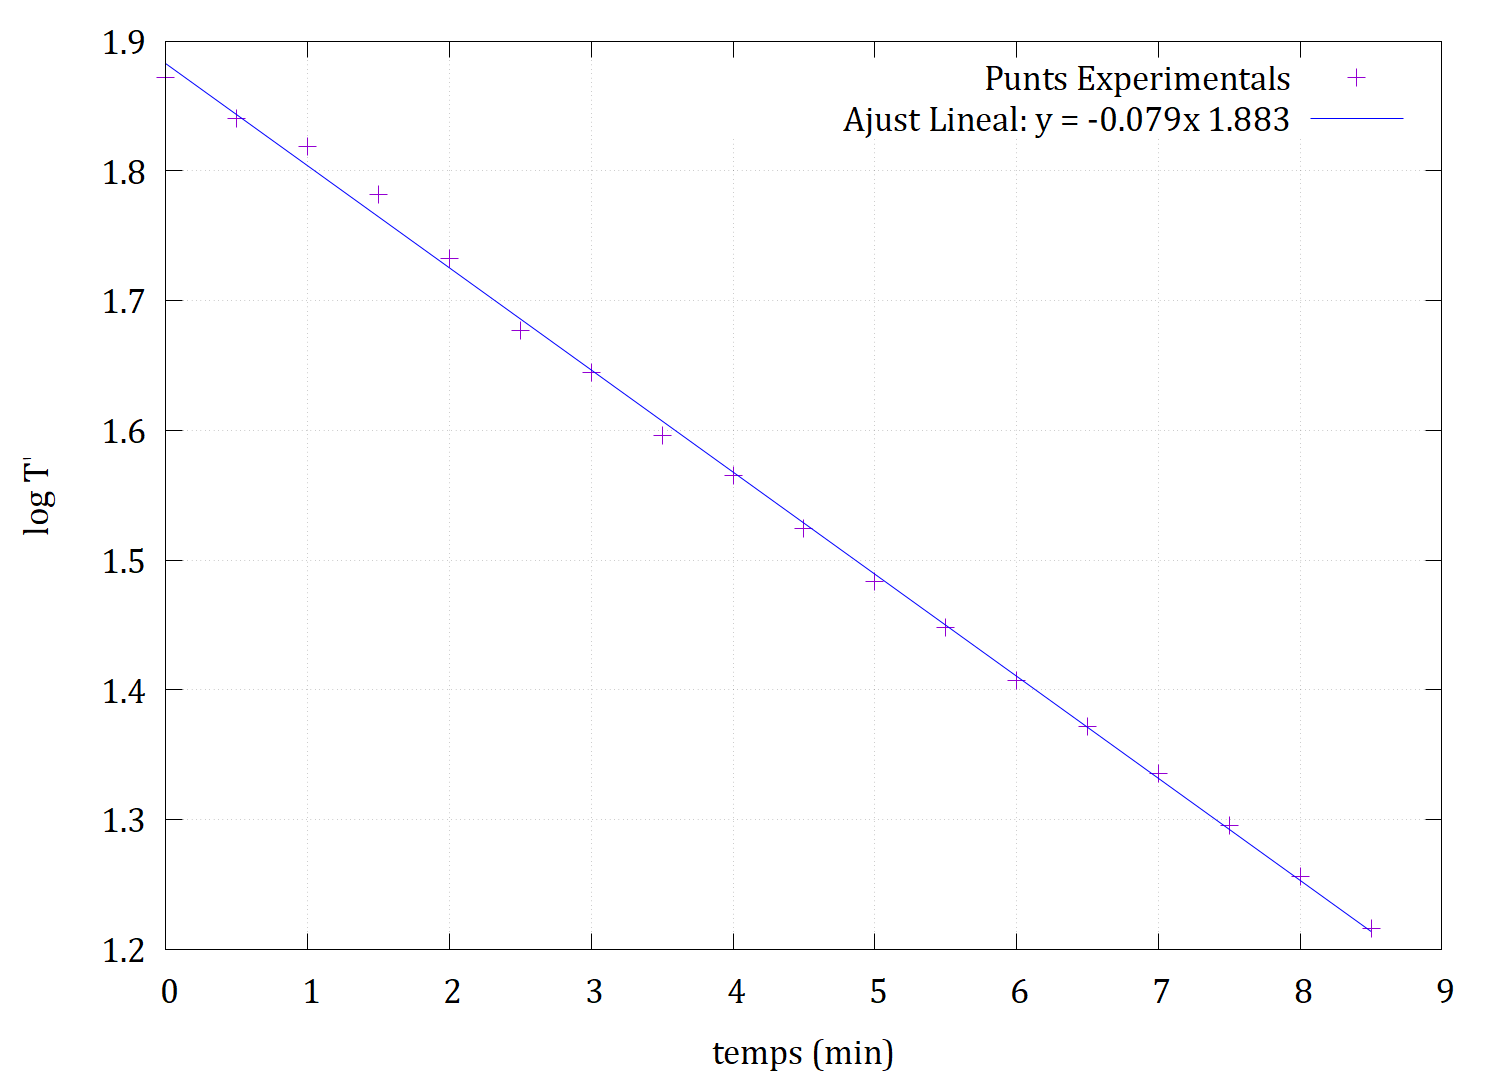
\includegraphics[width=0.45\linewidth]{ajustsemilog303.png}
    \caption{Gràfic semilogarítmic pel cabal 303,33 mL/min.}
    \label{fig4}
\end{figure}

Observem que obtenim unes rectes prou bones, fet que ens indica que les dades experimentals es comporten de forma similar a la predicció teòrica. Si, a més a més, comparem els valors de les pendents amb el valor esperat ${-Q_L}/{2,303V}$:

\begin{itemize}
    \item \textbf{Cabal 203,33 mL/min:} Obtenim un pendent teòric de \( -0,0546 \, \text{min}^{-1} \).
    \item \textbf{Cabal 253,33 mL/min:} Obtenim un pendent teòric de \( -0,0680 \, \text{min}^{-1} \).
    \item \textbf{Cabal 303,33 mL/min:} Obtenim un pendent teòric de \( -0,0815 \, \text{min}^{-1} \).
\end{itemize}

Així doncs, observem que els valors del pendent es desvien lleugerament dels esperats. Tanmateix, aquesta desviació la podem atribuir a errors experimentals i, donat que els valors resegueixen un comportament similar a l'esperat, podem assumir que les nostres dades segueixen la predicció teòrica.


\section{Conclusions}
En aquesta pràctica hem pogut comprovar que les equacions del balanç d'energia descriuen correctament el funcionament d'un sistema real, observant que, tal com anticipava la teoria, la temperatura decau exponencialment en funció del temps. A més hem pogut comprovar que els valors calculats de temps de residència s'adapten prou bé als temps teòrics si tenim en compte una certa desviació deguda a factors experimentals.

En conclusió, aquest experiment serveix per corroborar la validesa de les expressions teòriques del balanç d'energia ja que els valors experimentals són consistents amb els valors teòrics esperats. 


\newpage
\appendix
{\Huge \textbf{Annexos}}

\section{Calibratge de la bomba d'entrada}
L'objectiu del calibratge és trobar per a quins valors de rpm aconseguim treballar a uns cabals de 200 $\frac{\text{mL}}{\text{min}}$, 250 $\frac{\text{mL}}{\text{min}}$ i 300 $\frac{\text{mL}}{\text{min}}$. 

Per calibrar la bomba hem fet un seguit de mesures dels volums omplits per aquesta corresponents a una serie de valors de revolucions per minut (rpm) en un temps $t = 3$ min. Els valors obtinguts es poden veure a \ref{fig1}.

L'equació obtinguda amb els nostres punts experimentals és $y=7,0893x-16,071$, amb una $R^2 = 0,9995$, valor que ens indica que les nostres mesures tenen una bona correlació lineal.

A partir d'aquí calculem els cabals corresponents a cada valor de revolucions per minut usant que

\begin{equation}
    Q_L = \frac{V}{t}
\end{equation}

on, de nou, $t=3$ min. Amb això fàcilment es pot determinar que els valors de rpm de la bomba necessaris per treballar a uns cabals de 200 $\frac{\text{mL}}{\text{min}}$, 250 $\frac{\text{mL}}{\text{min}}$ i 300 $\frac{\text{mL}}{\text{min}}$ són els donats a la taula \ref{tab1}.

\section{Mesura del volum del tanc}
Per tal de mesurar el volum del tanc amb el que hem treballat hem usat dos mètodes distints, tenint cura que les condicions de mesura eren exactament les condicions d'operació del tanc (agitador connectat al 10$\%$ de la seva potència màxima, sense xocar amb les parets del recipient i a una alçada fixada). Les dues metologies han estat:
\begin{enumerate}
    \item Omplir el tanc amb aigua i connectar la bomba de sortida. Quan la quantitat d'aigua que surt pel cabal de sortida és zero, mesurar tot el volum contingut al recipient (usant material volumètric del laboratori).
    \item Amb el tanc buit, connectar les bombes d'entrada i sortida. Mesurar el temps que triga a omplir-se el reactor. Amb aquest temps i el cabal (que és conegut, donat el valor de rpm de la bomba), es pot determinar $V$ usant
    \begin{equation}
        V = Q_L \cdot t
    \end{equation}
\end{enumerate}
El resultats obtinguts amb cada mètode es poden veure a la corresponent secció d'aquest informe.

\section{Presa de dades experimentals}
Per tal de trobar les temperatures de sortida usant els diferents cabals proposats pel guió, hem efectuat mesures de la temperatura a dins del tanc, que prèviament havia estat omplert amb aigua a 90 ºC, cada 30 segons durant els primers 5 minuts i després cada minut, fins que la temperatura del tanc ha estat uns 10-15 ºC superior a la del tanc pulmó.

\section{Enllaç al Repositori de \textit{GitHub}}
A continuació adjuntem l'enllaç al repositori de \textit{GitHub} on podeu trobar el codi per representar les gràfiques usant \textit{Fortran} i \textit{Gnuplot}: \url{https://github.com/isaacbg25/labfeq}.

\end{document}